\exam{Teste 1 Desconhecido}
\question{Pergunta 1}
\begin{equation*}
	f(x)=e^{0.7x}-x^2-0.5
\end{equation*}
\textbf{(1)}
\begin{center} 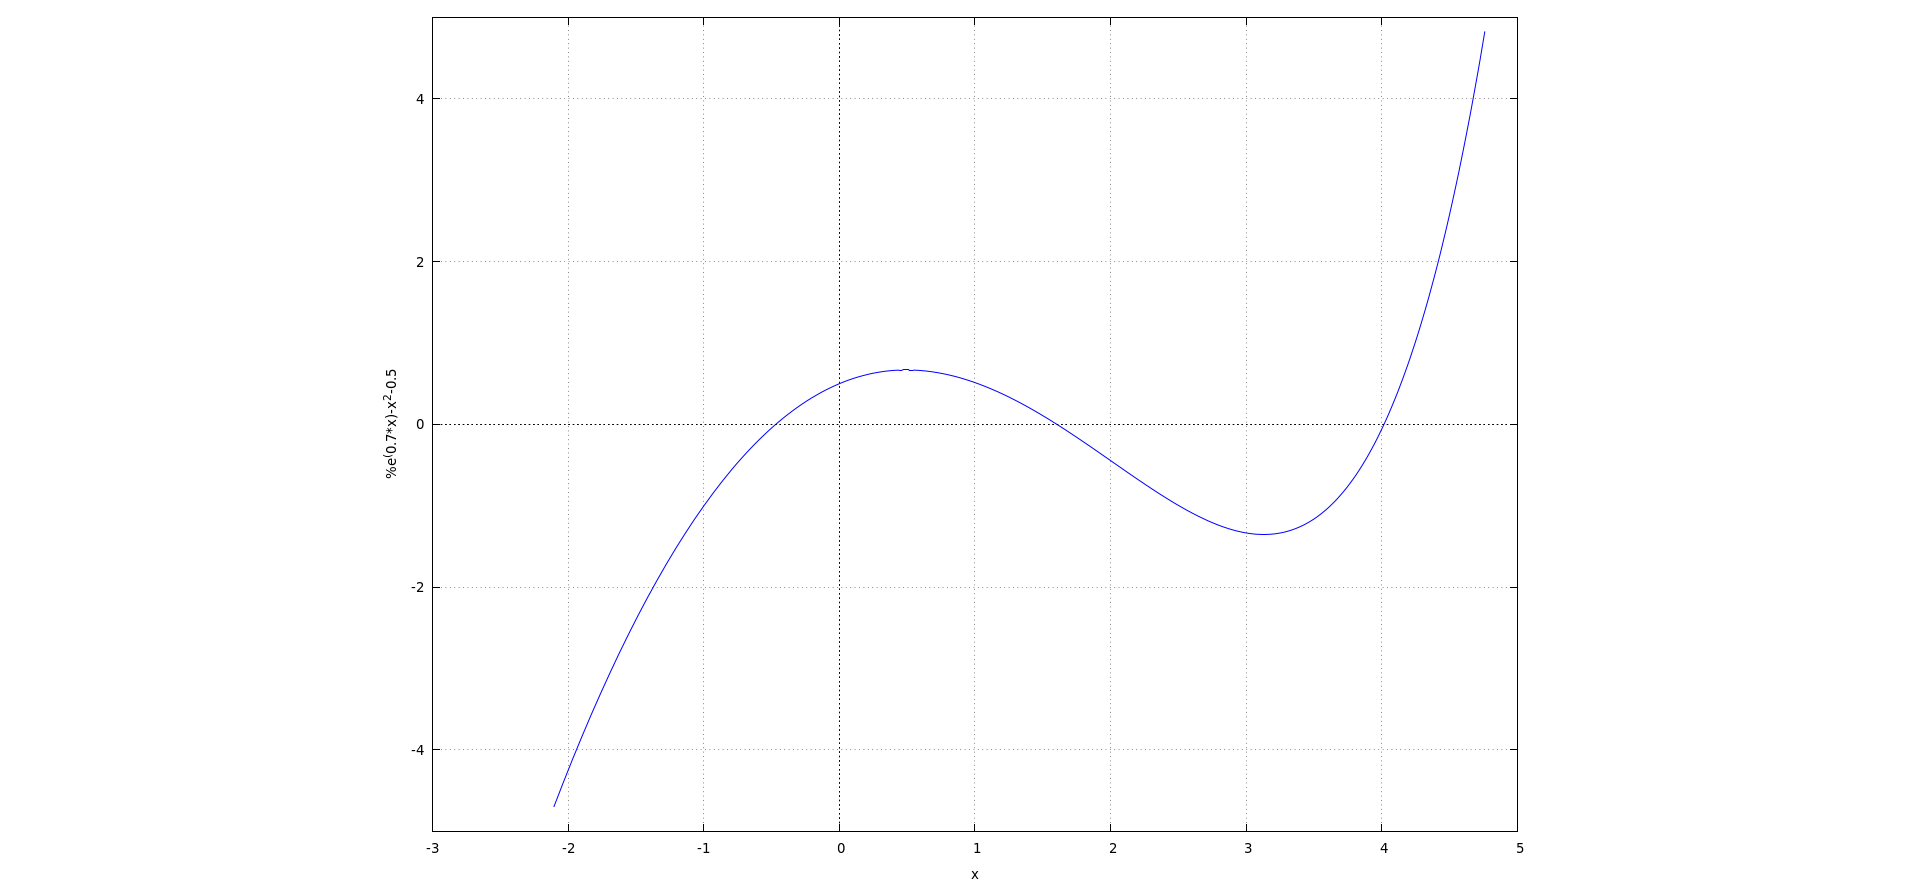
\includegraphics[height=60mm,keepaspectratio]{DESC1T1-1-1} \end{center}
A função possui três zeros.\\
\textbf{(2)} A maior raiz real positiva encontra-se no intervalo $[3,5]$.\\
\textbf{(3)}
\begin{center}
\begin{tabular}{c c c | c c c}
	$a$    & $b$    & $m$    & $f(a)$ & $f(b)$ & $f(m)$ \\ \hline
	-1.000 & 0.000  & -0.500 & -1.003 & 0.500  & -0.045 \\
	-0.500 & 0.000  & -0.250 & -0.045 & 0.500  & 0.277  \\
	-0.500 & -0.250 & -0.375 &        &        &
\end{tabular}
\end{center}
\textbf{(4)} Os cálculos permitem apresentar os resultados com três casas decimais, uma vez que os dados de entrada possuem também três casas decimais, e não ocorrem divisões (sendo que se considera que, por cada divisão, é retirada uma casa decimal ao resultado).\\
\textbf{(5)} Se o processo fosse dado por terminado na última iteração representada, o valor estimado da raiz seria $-0.375$, e o erro absoluto a diferença máxima em relação a ambos os extremos do intervalo. Assim, $\varepsilon_x=|-0.375-(-0.500)|=|-0.375-(-0.250)|=0.125$.

\question{Pergunta 2}
\begin{equation*}
	\begin{cases}
		f_1(x,y)=x^2-y-a=0\\
		f_2(x,y)=-x+y^2-b=0
	\end{cases}
	\implies
	\mathbf{J}=\begin{bmatrix}
  		f_{1,x}' & f_{1,y}'\\
  		f_{2,x}' & f_{2,y}'
	\end{bmatrix}=\begin{bmatrix}
  		2x & -1\\
  		-1 & 2y
	\end{bmatrix}
	\implies
	|\mathbf{J}|=4xy-1
\end{equation*}
\begin{alignat*}{4}
	h&=-\frac{
		\begin{vmatrix}
			f_1 & f_{1,y}' \\
			f_2 & f_{2,y}'
		\end{vmatrix}}
		{|\mathbf{J}|}
	   &&=-\frac{
		\begin{vmatrix}
			x^2-y-a  & -1 \\
			-x-y^2-b & 2y
		\end{vmatrix}}
		{|\mathbf{J}|}
	   &&=-\frac{2x^2y-x-y^2-2ay-b}{4xy-1}
	   &&=\frac{-2x^2y+x+y^2+2ay+b}{4xy-1} \\
	k&=-\frac{
		\begin{vmatrix}
			f_{1,x}' & f_1 \\
			f_{2,x}' & f_2
		\end{vmatrix}}
		{|\mathbf{J}|}
	   &&=-\frac{
		\begin{vmatrix}
			2x & x^2-y-a \\
			-1 & -x-y^2-b
		\end{vmatrix}}
		{|\mathbf{J}|}
	   &&=-\frac{2xy^2-y-x^2-2bx-a}{4xy-1}
	   &&=\frac{-2xy^2+y+x^2+2bx+a}{4xy-1}
\end{alignat*}
\begin{equation*}
	\begin{cases}
		x'=x+h\\
		y'=y+k
	\end{cases}
	\iff
	\begin{cases}
		x'=x+\dfrac{-2x^2y+x+y^2+2ay+b}{4xy-1}\\[1em]
		y'=y+\dfrac{-2xy^2+y+x^2+2bx+a}{4xy-1}
	\end{cases}
	\iff
	\begin{cases}
		x'=\dfrac{2x^2y+y^2+2ay+b}{4xy-1}\\[1em]
		y'=\dfrac{2xy^2+x^2+2bx+a}{4xy-1}
	\end{cases}
\end{equation*}
\begin{equation*}
	\begin{cases}
		a=1.2\\
		b=0.5
	\end{cases}
	\implies
	\begin{cases}
		x'=\dfrac{2x^2y+y^2+2.4y+0.5}{4xy-1}\\[1em]
		y'=\dfrac{2xy^2+x^2+x+1.2}{4xy-1}
	\end{cases}
\end{equation*}
Utilizando uma folha de cálculo, chega-se aos seguintes valores:
\begin{center}
\begin{tabular}{c | c}
	$x_n$ & $y_n$ \\ \hline
	1.10000 & 1.10000\\
	1.82604 & 1.60729\\
	1.64430 & 1.47070
\end{tabular}
\end{center}
\question{Pergunta 3}
\textbf{(a)} O método implementado é o método da tangente, uma vez que a cada iteração se calcula $x_{n+1}=x_n-f(x)/f'(x)$, em que $f(x) = x^3-a$ e $f'(x)=\partial f/\partial x=3x^2$.\\
\textbf{(b)} O critério de paragem funciona, mas exige que nenhum valor da sucessão seja $\approx 0$, uma vez que este valor produz grandes erros no cálculo de $x_{n+1}$ (se $x_n=0$, a tangente no ponto é horizontal, pelo que a tangente não interseta o eixo das abcissas num só ponto).
\begin{center} 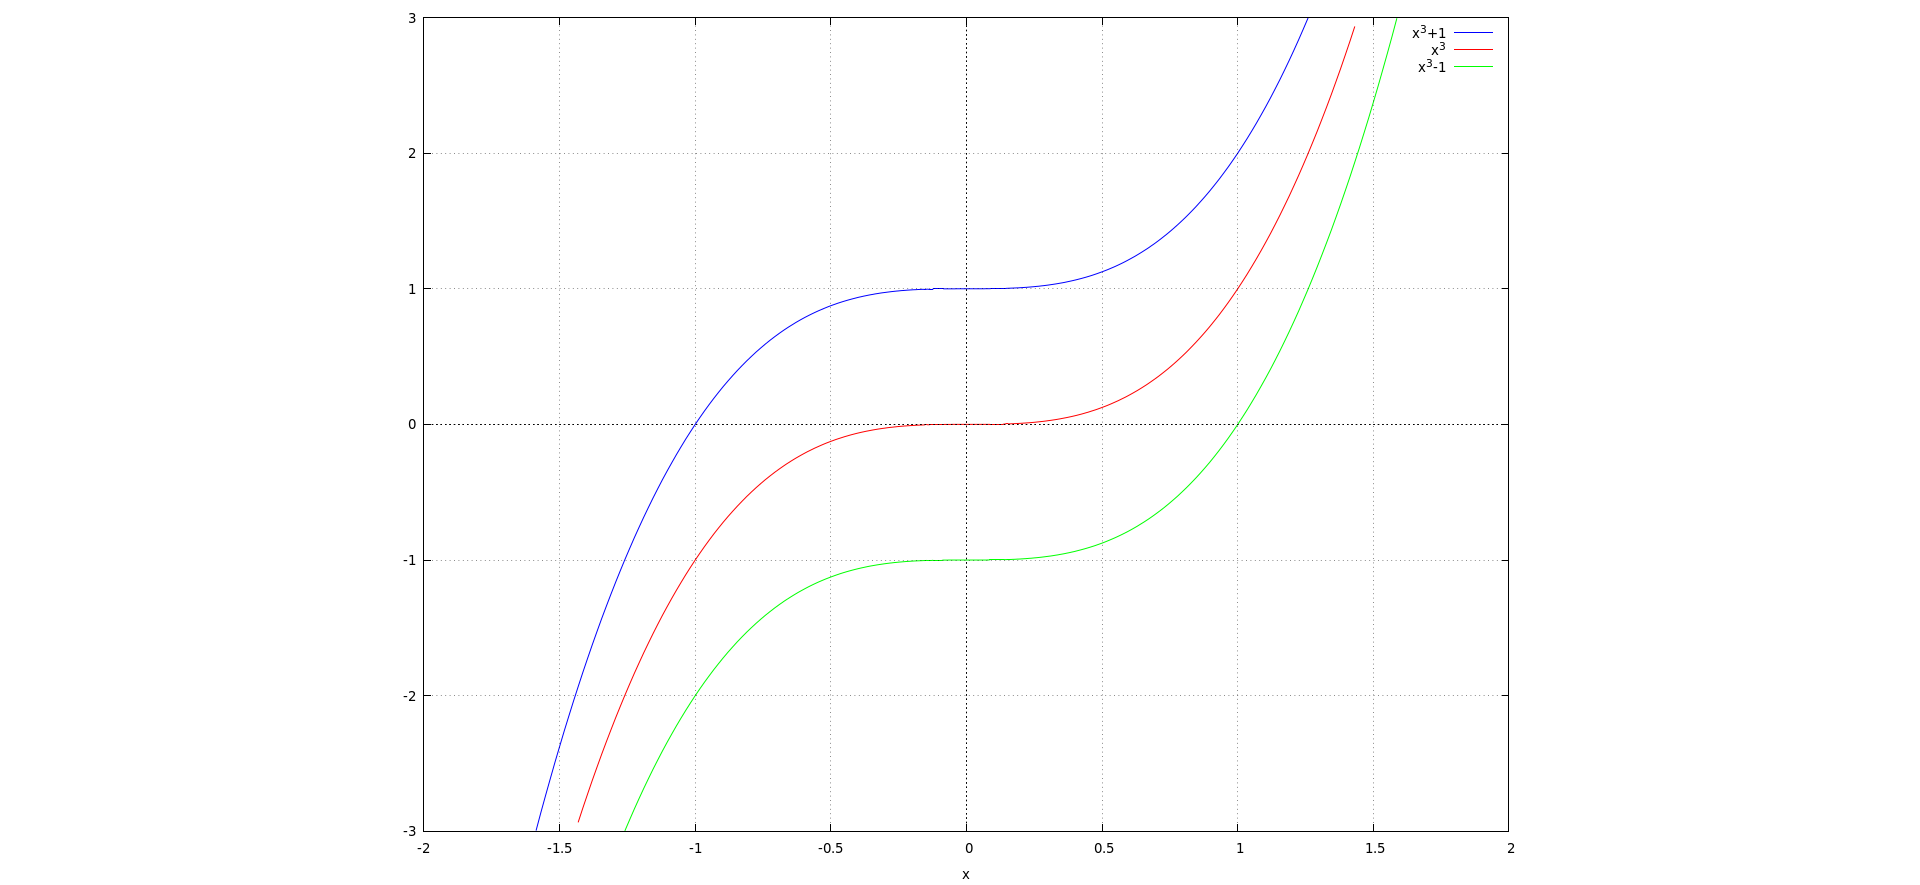
\includegraphics[height=60mm,keepaspectratio]{DESC1T1-3-b} \end{center}
\question{Pergunta 5}
A expressão recursiva para aplicação do método de Picard-Peano é
\begin{equation*}
	x_{n+1} \leftarrow \cot(x_n)\sin(3x_n)-4.9
\end{equation*}
que pode ser reformulada para corresponder a
\begin{alignat*}{1}
	g(x) &= \cot(x_n)\sin(3x_n)-4.9\\
	x_{n+1}&\leftarrow g(x_n)
\end{alignat*}
Vamos assim analizar a condição de convergência $|g'(x)| \leq 1$:
\begin{equation*}
	g'(x)=3\cot(x)\cos(3x)-\csc^2(x)\sin(3x)
\end{equation*}
\begin{center} 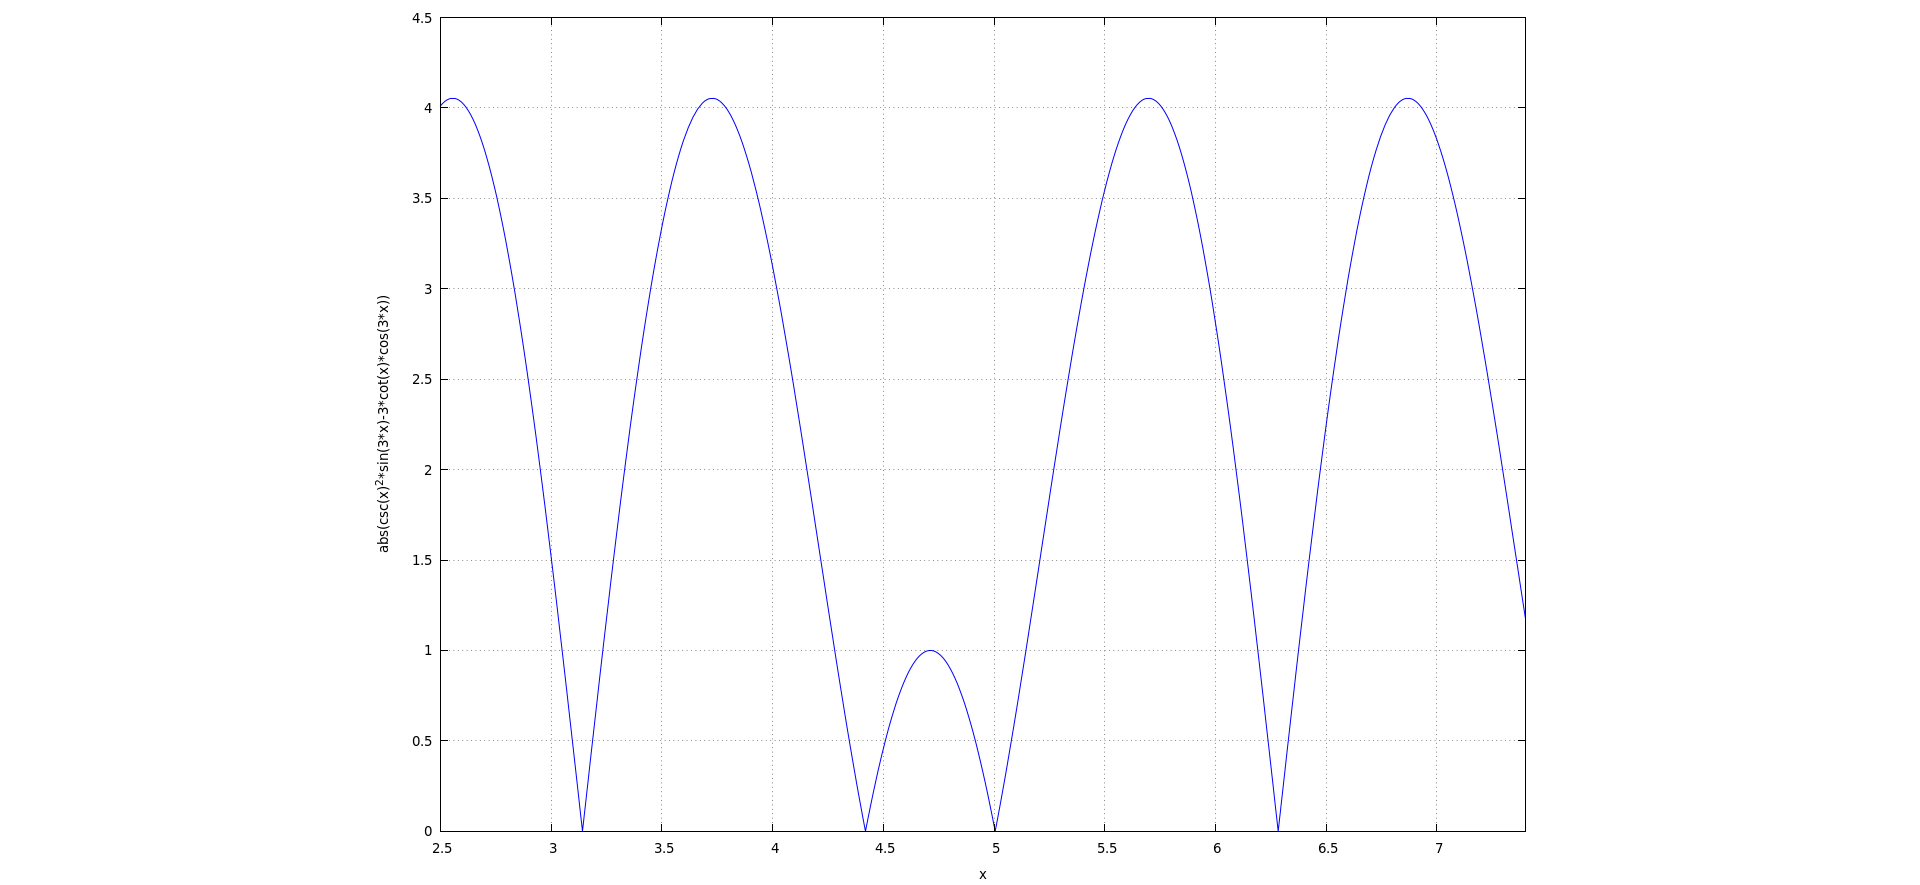
\includegraphics[height=60mm,keepaspectratio]{plotDESC1T1-5} \end{center}
Das opções disponíveis, apenas em $[4.5,5.1]$ se verifica $|g'(x)|\leq 1$.